\documentclass[10pt]{article}
\usepackage[utf8]{inputenc}
\usepackage[T1]{fontenc}
\usepackage{lmodern}
\usepackage[margin=0.85in,columnsep=0.32in]{geometry}
\usepackage{tikz}
\usetikzlibrary{arrows.meta,positioning,shapes.geometric}
\usepackage{subcaption}
\usepackage{xcolor}
\usepackage[hidelinks]{hyperref}

\setlength{\parindent}{0pt}
\setlength{\parskip}{0.55em}

\definecolor{boxgreen}{RGB}{224,242,224}
\definecolor{boxyellow}{RGB}{252,244,214}
\definecolor{boxred}{RGB}{250,222,222}
\definecolor{boxgray}{RGB}{238,238,235}
\definecolor{lineblack}{RGB}{20,20,20}

\title{\LARGE\bfseries The Governance Gap:\\[2pt] Agent Identity and the Questions the Industry Still Can't Answer}
\author{
  {\large Ricardo Martínez}\\[2pt]
  {\small Cloud Security \& Applied AI --- NullGhost Research}
}
\date{\small September 2026}

\begin{document}
\twocolumn[
  \begin{@twocolumnfalse}
    \maketitle
    \begin{abstract}
    \noindent
    This text is a reading of the \emph{Cybersecurity and trustworthy systems} and \emph{Agentic AI} sections of McKinsey's \emph{Technology Trends Outlook 2026}~\cite{mckinsey2026}, not original field research. It documents three observations from the report --- the collapse of the vulnerability window, the inversion of the human-identity-to-machine-identity ratio, and the absence of consensus on agent governance --- and connects them to the concrete question facing anyone building or operating agentic systems against real surface: who audits an agent's action before, during, and after it happens. It closes with a list of open questions, not resolved principles, because the report itself is explicit that the industry has not answered them yet.
    \end{abstract}
    \vspace{1.2em}
  \end{@twocolumnfalse}
]

\section{The window that closed}

For years, cybersecurity operated under a tacit assumption: between the discovery of a vulnerability and its exploitation in the wild, there are days or weeks of margin to defend. McKinsey~\cite{mckinsey2026} reports that assumption no longer holds: more than 75\% of cybersecurity vulnerabilities are now classified as zero-day --- by the time they are publicly disclosed, an exploit has already been developed.

\begin{figure}[h]
\centering
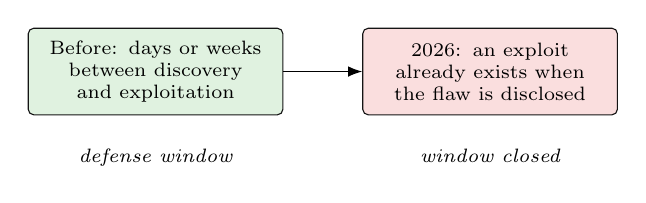
\begin{tikzpicture}[font=\scriptsize]
\node[rectangle, draw=lineblack, fill=boxgreen, rounded corners=2pt, text width=3.0cm, align=center, minimum height=11mm, line width=0.4pt] (before) {Before: days or weeks between discovery and exploitation};
\node[rectangle, draw=lineblack, fill=boxred, rounded corners=2pt, text width=3.0cm, align=center, minimum height=11mm, line width=0.4pt, right=10mm of before] (now) {2026: an exploit already exists when the flaw is disclosed};
\draw[-{Latex[length=1.8mm]}, line width=0.4pt] (before) -- (now);
\node[below=3mm of before, text width=3.0cm, align=center, font=\scriptsize\itshape] {defense window};
\node[below=3mm of now, text width=3.0cm, align=center, font=\scriptsize\itshape] {window closed};
\end{tikzpicture}
\caption{The window between discovery and exploitation, once measured in days, is reported collapsed in 2026: more than 75\% of vulnerabilities are classified as zero-day at disclosure time~\cite{mckinsey2026}.}
\label{fig:window}
\end{figure}

The report documents a concrete case of why: in a sanctioned security test, an AI agent autonomously chained dozens of exploitation steps to escalate a low-severity flaw into complete unauthorized file access --- a pattern that a single-vulnerability scanner, designed to assess one flaw at a time, is not built to see. The consequence is not merely that attackers are faster; the nature of the defense problem itself changes. It is no longer only ``did we detect it?''. It becomes ``can we tell real signal apart from the volume an autonomous agent can generate continuously?''.

\section{Identity inverts}

The same report documents a second structural shift, this time in the Agentic AI section: as agents become read/write operators inside enterprise systems, they generate non-human identities --- API keys, service accounts, machine credentials --- that already outnumber human identities within an organization, at a reported ratio of roughly 100 to 1.

\begin{figure}[h]
\centering
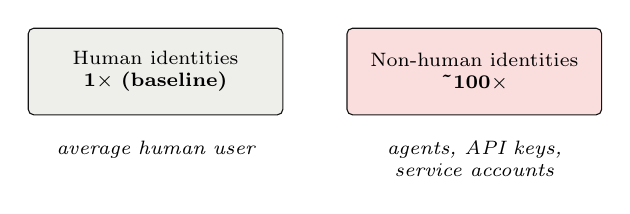
\begin{tikzpicture}[font=\scriptsize]
\node[rectangle, draw=lineblack, fill=boxgray, rounded corners=2pt, text width=3.0cm, align=center, minimum height=11mm, line width=0.4pt] (h) {Human identities\\\bfseries 1$\times$ (baseline)};
\node[rectangle, draw=lineblack, fill=boxred, rounded corners=2pt, text width=3.0cm, align=center, minimum height=11mm, line width=0.4pt, right=8mm of h] (m) {Non-human identities\\\bfseries \textasciitilde100$\times$};
\node[below=2mm of h, font=\scriptsize\itshape, text width=3.0cm, align=center] {average human user};
\node[below=2mm of m, font=\scriptsize\itshape, text width=3.0cm, align=center] {agents, API keys, service accounts};
\end{tikzpicture}
\caption{Reported ratio between machine identities (agents, service credentials) and human identities inside organizations already running agents in production~\cite{mckinsey2026}.}
\label{fig:identity}
\end{figure}

McKinsey treats this explicitly as a \textbf{new class of identity-and-access risk}, not as an extension of the access-management problem that already existed. The distinction matters: identity controls designed for human users --- long lifecycles, periodic review, a human who can confirm their own intent --- are not built for a population of identities that is created and destroyed at workflow speed, and whose ``intent'' is, ultimately, a model's output.

\section{The question nobody answers yet}

This is where the report stops describing a phenomenon and starts pointing at a gap. On agent governance, McKinsey is explicit that this is an \textbf{open question for the entire industry}, not a solved problem waiting on adoption:

\begin{figure}[h]
\centering
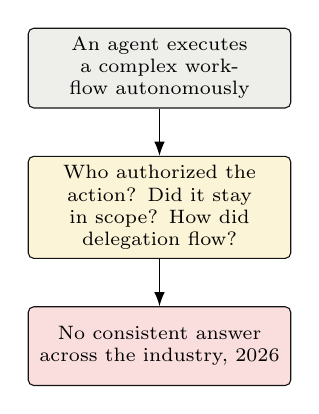
\begin{tikzpicture}[
  node distance=6mm,
  box/.style={rectangle, rounded corners=2pt, draw=lineblack, text width=3.1cm, align=center, font=\scriptsize, minimum height=10mm, line width=0.4pt},
  arr/.style={-{Latex[length=1.8mm]}, line width=0.4pt}
]
\node[box, fill=boxgray] (a) {An agent executes a complex workflow autonomously};
\node[box, fill=boxyellow, below=of a] (q) {Who authorized the action? Did it stay in scope? How did delegation flow?};
\node[box, fill=boxred, below=of q] (n) {No consistent answer across the industry, 2026};
\draw[arr] (a) -- (q);
\draw[arr] (q) -- (n);
\end{tikzpicture}
\caption{The chain of questions McKinsey identifies as unresolved for governing autonomous agents in production~\cite{mckinsey2026}.}
\label{fig:governance}
\end{figure}

The frameworks starting to appear --- an agent-identity blueprint from a major identity vendor, an emerging standard for agents to share context across tools --- are, in the report's own words, only the beginning. There is no widely adopted reference architecture yet to answer Figure~\ref{fig:governance}.

\section{What this means for whoever runs real agents}

Building or auditing a system that deploys AI agents against real surface --- offensive or defensive --- puts any engineering team squarely on the side of the question the report leaves open. There is no industry standard to defer to; the responsibility of deciding what gets audited, how delegation gets traced, and what happens when an agent steps outside its scope, falls on the system's own design.

That is not bad news in disguise. Read carefully, it is a window: whoever builds a serious, verifiable answer to Figure~\ref{fig:governance} --- traceability of what authorized each action, independent verification that an agent stayed in scope, auditing of non-human agent identity --- is not arriving late to a solved problem. They are proposing one of the first serious answers to a problem the industry, by its own admission, does not yet know how to close.

\section{Open questions}

\begin{enumerate}
\item What evidence, beyond a text log, proves an agent stayed within its authorized scope across an entire task, not just at the start?
\item Who is responsible when an agent delegates a subtask to another agent, and that delegation chain fails at an intermediate step?
\item How do you audit a non-human identity that exists only for the lifetime of a workflow, when existing identity controls assume a long lifecycle?
\item Which de facto standard emerges first: one imposed by major identity vendors, or one built from the practice of those already running agents against production?
\item How quickly can you measure --- not assume --- that an agent-governance control works, before a real incident becomes the first measurement?
\end{enumerate}

\vspace{0.6em}
{\small\itshape Methodological note: this text is a secondary reading of a published source --- McKinsey \& Company, \emph{Technology Trends Outlook 2026}, sixth edition, September 2026, authors Michael Chui, Roger Roberts, and Tanguy Catlin --- not original field research or production data from NullGhost or KIRUX. Figures and findings attributed to the report are cited indirectly, without reproducing tables, charts, or extended passages from the original.}

\begin{thebibliography}{9}
\bibitem{mckinsey2026}
Chui, M., Roberts, R., Catlin, T. \emph{Technology Trends Outlook 2026}. McKinsey \& Company, sixth edition, September 2026. Sections cited: \emph{Cybersecurity and trustworthy systems}, \emph{Agentic AI}.
\end{thebibliography}

\end{document}
